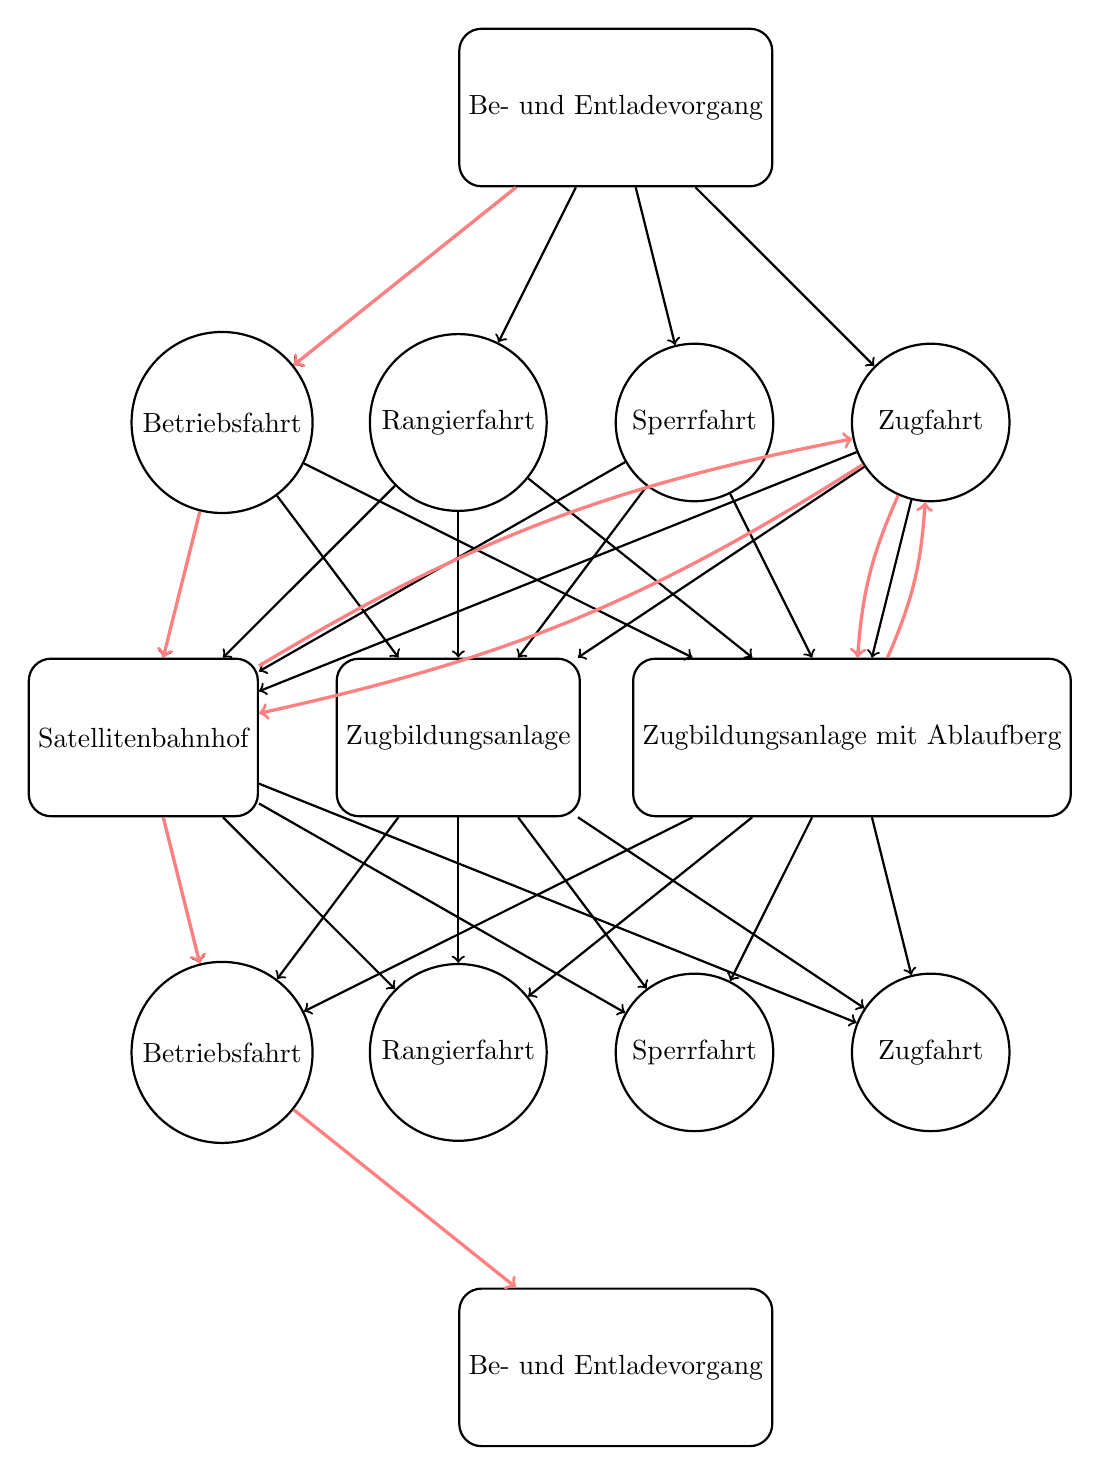
\begin{tikzpicture}
\node (BV) at (6,0) [rectangle, rounded corners=8pt,draw=black,fill=white,minimum size=20mm,thick] {Be- und Entladevorgang};
\node (BF) at (1,-4) [circle, rounded corners=8pt,draw=black,fill=white,minimum size=20mm, thick]
	{Betriebsfahrt};
\node (RF) at (4,-4) [circle, rounded corners=8pt,draw=black,fill=white,minimum size=20mm, thick]
	{Rangierfahrt};
\node (SF) at (7,-4) [circle, rounded corners=8pt,draw=black,fill=white,minimum size=20mm, thick]
	{Sperrfahrt};
\node (ZF) at (10,-4) [circle, rounded corners=8pt,draw=black,fill=white,minimum size=20mm, thick] {Zugfahrt};
\node (Sbf) at (0,-8) [rectangle, rounded corners=8pt,draw=black,fill=white,minimum size=20mm, thick] {Satellitenbahnhof};
\node (ZBA) at (4,-8) [rectangle, rounded corners=8pt,draw=black,fill=white,minimum size=20mm, thick] {Zugbildungsanlage};
\node (ZBAA) at (9,-8) [rectangle, rounded corners=8pt,draw=black,fill=white,minimum size=20mm, thick] {Zugbildungsanlage mit Ablaufberg};
\node (BF2) at (1,-12) [circle, rounded corners=8pt,draw=black,fill=white,minimum size=20mm, thick]
	{Betriebsfahrt};
\node (RF2) at (4,-12) [circle, rounded corners=8pt,draw=black,fill=white,minimum size=20mm, thick]
	{Rangierfahrt};
\node (SF2) at (7,-12) [circle, rounded corners=8pt,draw=black,fill=white,minimum size=20mm, thick]
	{Sperrfahrt};
\node (ZF2) at (10,-12) [circle, rounded corners=8pt,draw=black,fill=white,minimum size=20mm, thick] {Zugfahrt};
\node (BV2) at (6,-16) [rectangle, rounded corners=8pt,draw=black,fill=white,minimum size=20mm,thick] {Be- und Entladevorgang};

\draw[->, black!100, thick] (BV) to (BF);
\draw[->, black, thick] (BV) to (RF);
\draw[->, black, thick] (BV) to (SF);
\draw[->, black, thick] (BV) to (ZF);
\draw[->, black, thick] (BF) to (Sbf);
\draw[->, black, thick] (BF) to (ZBA);
\draw[->, black, thick] (BF) to (ZBAA);
\draw[->, black, thick] (RF) to (Sbf);
\draw[->, black, thick] (RF) to (ZBA);
\draw[->, black, thick] (RF) to (ZBAA);
\draw[->, black, thick] (SF) to (Sbf);
\draw[->, black, thick] (SF) to (ZBA);
\draw[->, black, thick] (SF) to (ZBAA);
\draw[->, black, thick] (ZF) to (Sbf);
\draw[->, black, thick] (ZF) to (ZBA);
\draw[->, black, thick] (ZF) to (ZBAA);
\draw[->, black, thick] (Sbf) to (BF2);
\draw[->, black, thick] (Sbf) to (RF2);
\draw[->, black, thick] (Sbf) to (SF2);
\draw[->, black, thick] (Sbf) to (ZF2);
\draw[->, black, thick] (ZBA) to (BF2);
\draw[->, black, thick] (ZBA) to (RF2);
\draw[->, black, thick] (ZBA) to (SF2);
\draw[->, black, thick] (ZBA) to (ZF2);
\draw[->, black, thick] (ZBAA) to (BF2);
\draw[->, black, thick] (ZBAA) to (RF2);
\draw[->, black, thick] (ZBAA) to (SF2);
\draw[->, black, thick] (ZBAA) to (ZF2);

\draw[->, red!50, very thick] (BV) to (BF);
\draw[->, red!50, very thick] (BF) to (Sbf);

\draw[->, red!50, very thick] (Sbf) to[bend left=10] (ZF);
\draw[->, red!50, very thick] (ZF) to[bend left=10] (Sbf);
\draw[->, red!50, very thick] (ZF) to[bend right=10] (ZBAA);
\draw[<-, red!50, very thick] (ZF) to[bend left=10] (ZBAA);

\draw[<-, red!50, very thick] (BF2) to (Sbf);
\draw[<-, red!50, very thick] (BV2) to (BF2);

\end{tikzpicture}